\documentclass{article}

% Language setting
% Replace `english' with e.g. `spanish' to change the document language
\usepackage[english]{babel}

% Set page size and margins
% Replace `letterpaper' with `a4paper' for UK/EU standard size
\usepackage[a4paper,top=2cm,bottom=2cm,left=3cm,right=3cm,marginparwidth=1.75cm]{geometry}

% Useful packages
\usepackage{amsmath}
\usepackage{graphicx}
\usepackage[colorlinks=true, allcolors=blue]{hyperref}

\title{Michaelis-Menten  Equation}
\author{BS22B001}

\begin{document}
\maketitle
\section{Introduction}

This a document that will explain Michaelis-Menten Equation that determines the order of reaction in Enzyme reaction

\section{BS22B001}
\subsection{Equation}

\begin{equation}
    V_0 = \frac{V_{max}[S]}{k_m+[S]}
\end{equation}
\footnotemark

\subsection{Explanation}

The Michaelis-Menten equation arises from the general equation for an enzymatic reaction:
E + S $\rightleftharpoons$  ES $\rightleftharpoons$  E + P, where E is the enzyme, S is the substrate, ES is the enzyme-substrate complex, and P is the product. Thus, the enzyme combines with the substrate in order to form the ES complex, which in turn converts to product while preserving the enzyme. The rate of the forward reaction from E + S to ES may be termed k1, and the reverse reaction as k-1. Likewise, for the reaction from the ES complex to E and P, the forward reaction rate is k2, and the reverse is k-2. Therefore, the ES complex may dissolve back into the enzyme and substrate, or move forward to form product. 


\begin{figure}
\centering
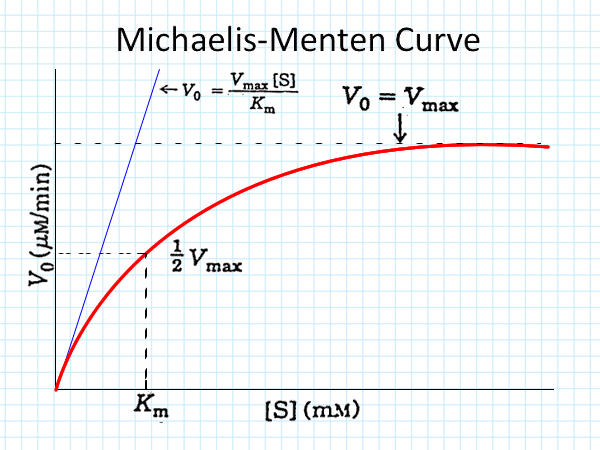
\includegraphics[width=0.4\textwidth]{2.png}
\caption{\label{fig:frog}This is a plot of .}
\end{figure}

Km is the Michaelis-Menten constant which shows the concentration of the substrate when the reaction velocity is equal to one half of the maximal velocity for the reaction. It can also be thought of as a measure of how well a substrate complexes with a given enzyme, otherwise known as its binding affinity. An equation with a low Km value indicates a large binding affinity, as the reaction will approach Vmax more rapidly. An equation with a high Km indicates that the enzyme does not bind as efficiently with the substrate, and Vmax will only be reached if the substrate concentration is high enough to saturate the enzyme.

As the concentration of substrates increases at constant enzyme concentration, the active sites on the protein will be occupied as the reaction is proceeding. When all the active sites have been occupied, the reaction is complete, which means that the enzyme is at its maximum capacity and increasing the concentration of substrate will not increase the rate of turnover. Here is an analogy which helps to understand this concept easier.

Vmax is equal to the product of the catalyst rate constant (kcat) and the concentration of the enzyme. The Michaelis-Menten equation can then be rewritten as V= Kcat [Enzyme] [S] / (Km + [S]). Kcat is equal to K2, and it measures the number of substrate molecules "turned over" by enzyme per second. The unit of Kcat is in 1/sec. The reciprocal of Kcat is then the time required by an enzyme to "turn over" a substrate molecule. The higher the Kcat is, the more substrates get turned over in one second.

Km is the concentration of substrates when the reaction reaches half of Vmax. A small Km indicates high affinity since it means the reaction can reach half of Vmax in a small number of substrate concentration. This small Km will approach Vmax more quickly than high Km value.

When Kcat/ Km, it gives us a measure of enzyme efficiency with a unit of 1/(Molarity*second)= L/ (mol*s). The enzyme efficiency can be increased as Kcat has high turnover and a small number of Km. 

Roll No:BS22B001
Name: Alan Royce Gabriel S
\footnotetext{https://en.wikibooks.org/wiki/Structural_Biochemistry/Enzyme/Michaelis_and_Menten_Equation}

\end{document}
